\section{Design of Acceleration Module}
\subsection{The Overview of FPGA Acceleration Framework}
\begin{figure*}[!ht]
    \centering
    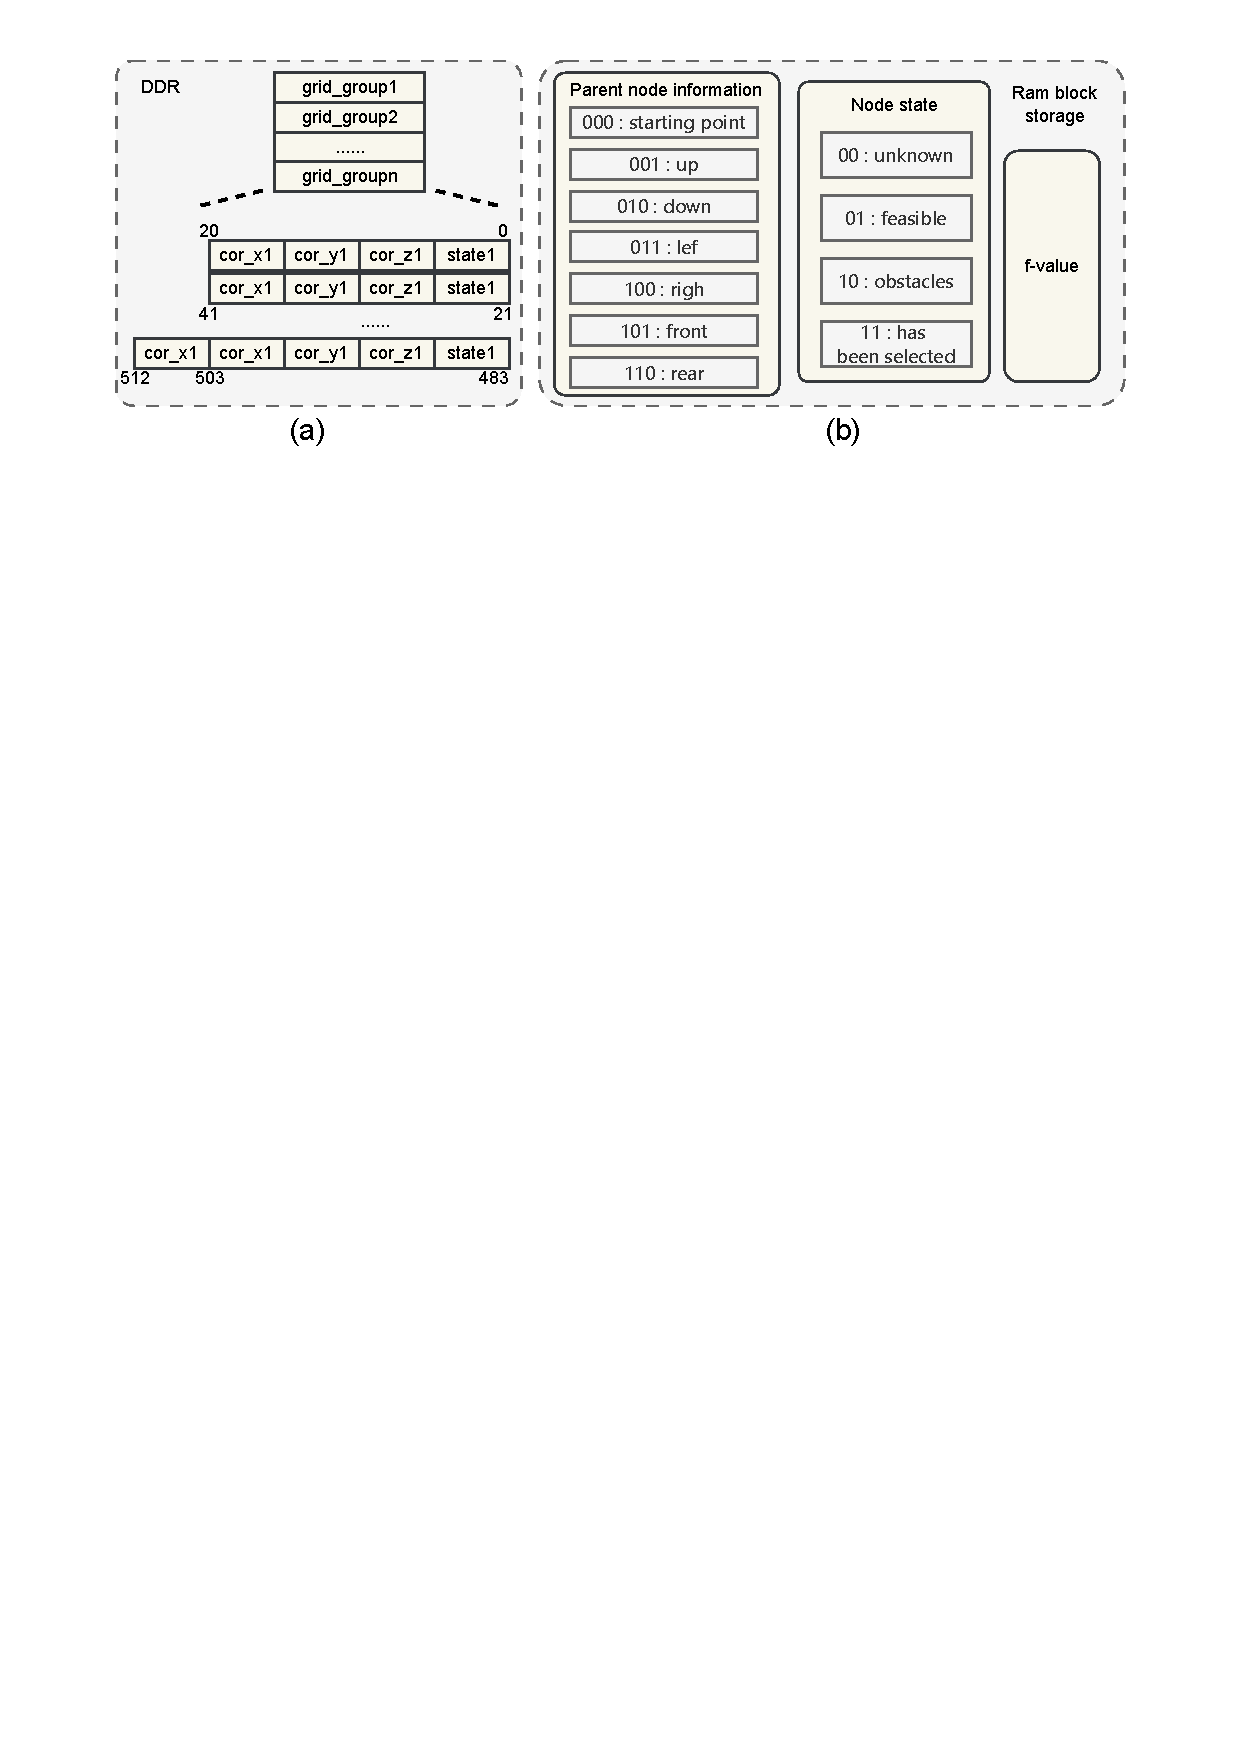
\includegraphics[width=\textwidth]{figures/acceleration/Data Arc.pdf}
    \caption{Data structure ON FPGA.(a)Data Layout in FPGA Memory DDR.(b)Storage format of multi-cRAM.}
\end{figure*}
Conventional implementations of A* search usually use two lists to store the states during its expansion, i.e., the \textbf{open list} and the \textbf{closed list}. 
The closed list stores all the visited states, and is used to prevent unnecessary repeated expansion of the same state. This list is often implemented by a linked hash table to detect the duplicated nodes. 
The open list normally stores the states whose successors have not been fully explored yet. The open list uses a priority queue as its data structure, typically implemented by a binary heap. 
States in the open list are sorted according to the function value of heuristic function f (x).


A lot of work proves that memory access is the time bottleneck of the algorithm compared to the computation time, as Figure~\ref{fig:Execution Time} shows.
So our work is dedicated to propose a FPGA-based implementation to accelerate the detailed routers, uses efficient memory access management and parallelism to achieve better performance.
Figure~\ref{fig:overview} shows the overview of FPGA acceleration framework.





\subsection{Cost\_Calculator Module}
Cost\_calculator module calculates the F-values of 6 peripheral points in parallel according to the input center point and surrounding point information.
The information in 6 directions is calculated in parallel to the Manhattan distance, and the F value of the 6 surrounding points is calculated based on F=G+H.

\begin{figure}[htbp]
    \centering
    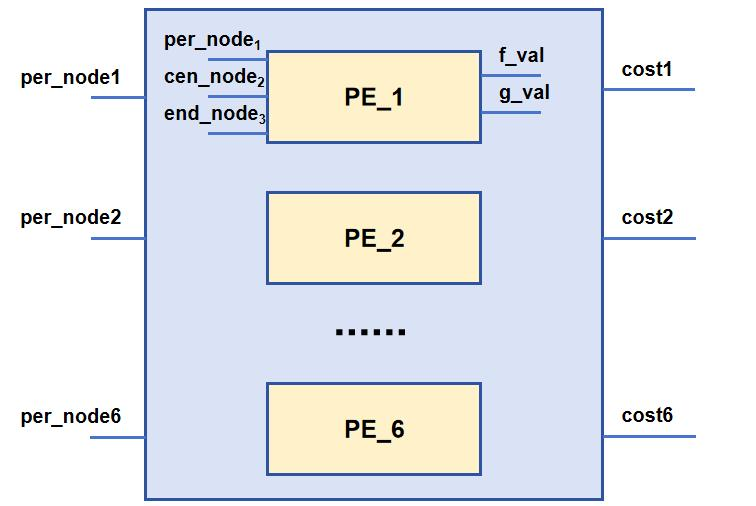
\includegraphics[width=8cm]{figures/acceleration/Cost Calculator Module.jpg}
    \caption{The Cost\_Calculator Module.}
\end{figure}


\subsection{Cost\_Cache Module}
\textbf{Instantiate multiple ram groups to store node information on the corresponding dimension.}Traditional FPGA-based path planning algorithms have significant bottlenecks in maintaining \textbf{open list} and \textbf{closed list}.
The dynamic sorting mechanism requires the storage structure to be reordered after each search iteration. This frequent sorting operation will not only consume a lot of programmable logic resources, but also produce a processing delay that does not match the hardware architecture, which seriously restricts the real-time performance of the system.
In addition, dynamic memory management of variable-length data structures leads to fragmented access to Block RAM, resulting in reduced hardware resource utilization.

To solve this problem we observed, the dimensional organization of RAM can be efficiently managed through hierarchical mapping, in FPGA-based storage architecture design, as fig1 shows.
For 2D data structure, row-priority storage strategy can be adopted, so that each RAM module can store the data node corresponding to the row (first dimension) independently.
When extended to a three-dimensional structure, each RAM module can be responsible for storing node information in a fixed plane, such as the third dimension.
Through the introduction of address mapping module, high-dimensional addresses (such as three-dimensional coordinates (x,y,z)) can be converted into two-dimensional storage addresses inside each RAM module. This hierarchical mapping mechanism significantly improves storage access efficiency and data throughput.





% \begin{table}[]
%     \centering
%     \caption{Ram block storage of node information in the corresponding dimension}
%     \begin{tabular}{|l|l|l|}
%     \hline
%     \multicolumn{1}{|c|}{\textbf{F}} & \multicolumn{1}{c|}{\textbf{Parent node information}} & \multicolumn{1}{c|}{\textbf{Node state}} \\ \hline
%                                       & 000 : starting point                                   & 00 : unknown                               \\ \hline
%                                       & 001 : up                                                & 01 : feasible                              \\ \hline
%                                       & 010 : down                                              & 10 : obstacles                             \\ \hline
%                                       & 011 : left                                              & 11 : has been selected                     \\ \hline
%                                       & 100 : right                                             &                                          \\ \hline
%                                       & 101 : front                                             &                                          \\ \hline
%                                       & 110 : rear                                              &                                          \\ \hline
%     \end{tabular}
%     \end{table}


\begin{figure}[htbp]
    \centering
    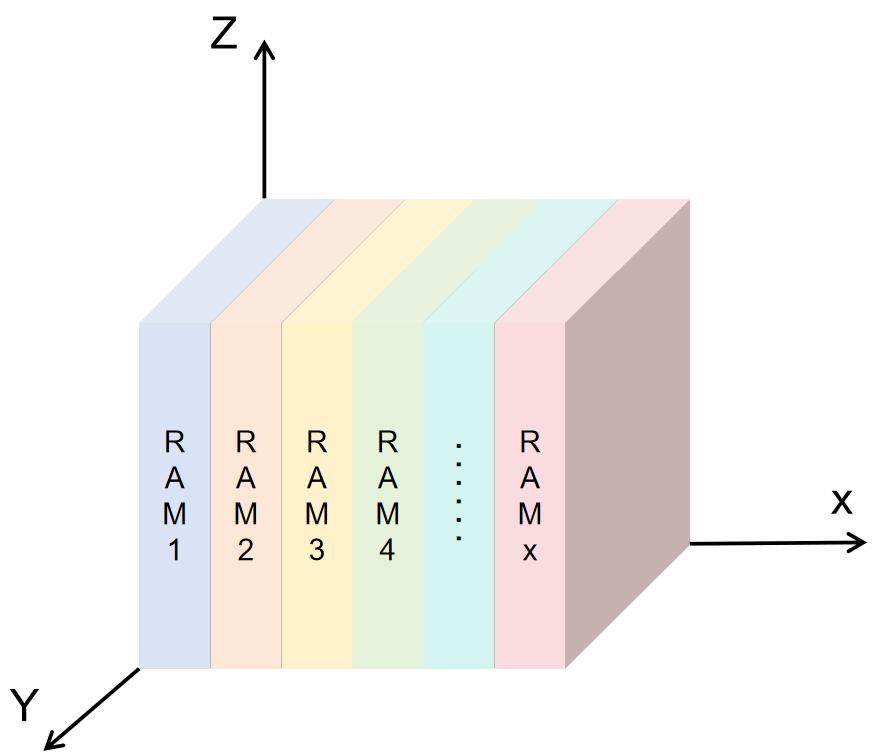
\includegraphics[width=8cm]{figures/acceleration/Cost Cache.jpg}
    \caption{Instantiate multiple ram block storage}
\end{figure}


\subsection{F-value update Module}
After the path cost calculation module completes the F-value generation of the adjacent nodes of the central node, the system executes the storage update process based on logical control.
First, Cost\_cache memory is accessed through the coordinate addressing mechanism to extract the status flag bit and historical F-value of the target node: If the flag bit is detected as the initial state (00), the new F-value and status flag are directly written without constraints;
If the status flag is explored state (01), the hardware comparator is triggered to perform the numerical relationship determination of the new F-value and the stored F-value in parallel, and the path cost validity check is performed at the same time to avoid calculation anomalies.
Finally, the storage unit is selectively updated according to the judgment result: for the initial state node to load new data completely, the explored state node only performs overwrite storage and synchronously updates the state when the new F-value is better.
This mechanism uses the state-driven conditional write strategy to reduce the redundant access to memory and data overwrite operations while maintaining the principle of path planning optimality.

\subsection{Minimum F-Value Sorting Module}
In the process of selecting the least cost node of distributed storage architecture, the system uses the hierarchical comparison mechanism of self-updating to realize the dynamic update of the center point.
The built-in hardware minimum value tracking module of each storage unit immediately triggers the parallel comparison circuit in the unit when a new F-value is detected: real-time comparison of the currently stored minimum F-value and the new written value through the special register group, dynamic update of the minimum cost value and its three-dimensional coordinate information, and generate an effective status flag bit to synchronize to the arbitration controller.
When the valid flag bits of all storage units are ready, the hierarchical comparison architecture starts the global arbitration in stages. First, the local minimum values in each storage row are screened in parallel by row-level comparator array, and then the row-level minimum values are progressively compared by a tree arbiter based on depth-first strategy. Finally, the coordinates and path cost values of the globally optimal nodes are output.

After the selected global minimum is verified, the system loads the new central point information into the path planning logic through the three-dimensional coordinate bus. At the same time, double buffer register group is used to realize the decoupling of the computing unit and the storage unit to ensure the continuous operation of the comparison pipeline during the data update cycle.
By means of distributed priority arbitration mechanism implemented by hardware, the architecture transforms the ergodic search in traditional algorithms into multilevel pipeline operation, which avoids the resource competition problem of centralized comparison architecture while maintaining real-time path planning.
% \section{Reduction Alternative PE Array Architecture}\label{sec:method1}

% \subsection{Challenge}

% Linear operation and element-wise operation are two dominating operations in Mamba.
% Linear operations like matrix multiplications are usually accelerated by Tensor Core, which is a domain specific architecture with the reduction tree.
% Due to the reduction of partial inner product, the linear operations exhibit extremely high compute intensity (\textit{e.g.}, $>$1000 FLOPs/Byte).
% However, as shown in Figure~\ref{fig:time_proportion}, the time proportion of element-wise operations escalates significantly as sequence length increases (\textit{e.g.}, $>$60\% with 2048 input length).
% Because the element-wise operations do not need reduction, applying them on Tensor Core-based architecture should introduce large amount of invalid computations, leading to an extreme inefficiency (\textit{e.g.}, 1/16 normalized speed). 
% We call it the incompatibility between element-wise operations and Tensor Core.

% \subsection{Motivation and Insights}

% Our motivation stems from the inefficiencies observed in element-wise computations on tensor cores. 
% Because the attention operations contain non-linear softmax, previous Transformer accelerators~\cite{wang2022via,lu2020hardware} employed independent hardware units to support both attention and linear operations. 
% In contrast, Mamba architecture only consists of linear operations, element-wise operations, and a few activation functions. 
% The only difference of linear of element-wise operations is whether execute reduction or not. 
% Recognizing this simplicity, \textbf{our key insight is that by disabling the reduction tree, the Tensor Core-based PE arrays can execute element-wise operations.}
% % Recognizing this simplicity, our key insight lies in the integration of hardware units capable of handling these dominant linear and element-wise operations, thereby maximizing hardware reuse.

% \subsection{Approach}
% \textbf{Reduction Alternative PE Arrays.}
% The reduction alternative processing element (PE) arrays support configurablility. 
% The reduction tree consists of 16 slices (taking 16 for instance) and operates in two modes: reduction mode for linear operations and non-reduction mode for element-wise operations. 
% In reduction mode, the reduction tree is enabled.
% For a 16-to-1 reduction tree slice, the outputs from 16$\times$1 PE arrays are fed into one reduction tree slice, which employs multi-level additions to compute the sum.
% In non-reduction mode, the reduction tree is enabled and the outputs from 16$\times$16 PE arrays skip the reduction directly. 
% In addition, the last-level addition in each slice supports three input to accumulate the partial results for linear operations.

% We define that a reconfigurable computing unit (RCU) consists of  16$\times$16 PE arrays and a reduction tree, as shown in Figure~\ref{fig:architecture} left. 
% Each reconfigurable PE (RPE) is configured to support three main computations with three data paths: a shift path for exponential function, a piecewise path for SiLU function, and a normal path for addition or multiplication. 
% The normal path contains a floating-point multiplier, a floating-point adder, and a multiplexer unit to handle element-wise multiplication and addition computations. 
 

% \textbf{Reconfigurable Computing Unit.}
% We provide a detailed explanation of how the RCU operates for the four specific computations in Mamba, as shown in Figure~\ref{fig:architecture} right.

% \textit{\underline{MM-RCU.}}
% The RCU is configured as a matrix multiplication mode (MM-RCU) to support linear operations. 
% The reduction tree in RCU and the floating-point multiplier units in RPE are enabled. 
% Therefore, for a matrix multiplication operation of two matrices of size 16$\times$16, the results calculated by the 16$\times$16 array of multipliers are then passed through the reduction tree to produce 16 final results. 
% Then, this process is repeated totally 16 times to obtain the complete result of the 16$\times$16 matrix multiplication. 
% To support the accumulation of partial sums, an additional adder is added at the final level of the reduction tree.

% \textit{\underline{EW-RCU.}}
% When RCU is configured as element-wise mode (EW-RCU), the reduction tree is disabled, while the P2D buffer is enabled, and the floating-point multiplier or adder units in RPE are activated. 
% For an element-wise multiplication operation of two 16x16 matrices, the results calculated by the 16$\times$16 array of RPEs maintains the same dimensions of 16$\times$16 and are output to the buffer in parallel.
% % After 16 clock cycles, the results are sequentially written out.

% \textit{\underline{EXP-RCU.}}
% When RCU is configured as exponential mode (EXP-RCU), the reduction tree is disabled. 
% The floating-point multiplier, adder units, and exponential shift unit in RPE are enabled. 
% Therefore, for a 16$\times$16 matrix performing exponential function operation, the RCU first executes element-wise multiplication by using the multipliers, then executes element-wise addition by using the adders. 
% Afterward, the exponential shift unit performs a logic operation, a shift operation and a biased operation to obtain the final output, as shown in Figure~\ref{fig:overview} right bottom.

% \textit{\underline{SiLU-RCU.}}
% When RCU is configured as SiLU mode (SiLU-RCU), the floating-point multiplier or adder, the range detector, and the constant output unit in RPE are enabled while the reduction tree is disabled.
% For a 16$\times$16 input matrix, each input is first distinguished by range, and then depending on the difference of range, each input is processed by employing either the constant output or normal element-wise computations.
% The SiLU-RCU decomposes the SiLU operation into 0, 2, or 4 instances of element-wise operations according to equation~\ref{eq:silu_approx}.
